\documentclass[../index.tex]{subfiles}

\begin{document}

\chapter{SYSTEM DEVELOPMENT METHODOLOGY}

This chapter will define the development methodology which acts as a guideline to fulfil the goals
and objectives of the project. The selected methodology will be justified based on how the
methodology will help the development of the project. It will be followed by the explanation of the
phases of the selected methodology. Then, the system requirements will be analysed in order to be
able to develop a reliable system. The chapter will be ended by the conclusion of the previous
discussion regarding the selected methodology, development phases based on the selected methodology,
and system requirement analysis for the project development.

\section{Methodology Selection and Justification}

The primary objective of this project is to successfully develop a hardware firewall which home
users can use to secure their local network. As this project will only involves infrastructure
design, system integration, and configuration of existing software and technology without any
application development, the waterfall model is selected as the development methodology. Waterfall
model is selected as the proposed system will mainly serve its function with minimal user-facing
interface. This is in accordance with the definition of waterfall model where the product definition
is required to be stable among the course of the development. Another reason is the project involves
hardware development or configuration where manufacturing or procurement cost are involved. In
addition, the developed system appliance could be considered as critical system which requires
extensive safety and security analysis of the solution specification and design
\cite{balaji2012waterfall}.

\section{Phases of Selected Methodology}

The Waterfall model is a linear and sequential software development process consisting of several
phases. The Waterfall model initiated with Requirement Gathering and Analysis, followed by System
Design, Implementation, Integration and System Testing, and ended with Deployment and Maintenance.

\subsection{Requirements Gathering and Analysis}

The Waterfall project methodology is started by gathering the project requirements and analyse the
collected facts. The system services, constraints, and objectives are established with the system
users. They are then defined in detail and serve as a system specification.

For this project, this phase will discuss several network security concerns that exist in home
network environment. After the issues and concerns have been identified, the possible solution or
countermeasures will be discussed. The outcome of the discussion for this phase should be used as
the reference for considerations and justifications in later phases.

This project has gathered the potential issues that exist in home network environment in Chapter 1
and further discussed it in Chapter 2. Followed by that, the possible solution and improvement of
the gathered issues and concerns has been explored. The outcome of the discussion for this phase
will be used as the reference for considerations and justifications in following system development
phases.

\subsection{System Design}

Following the Requirements Gathering and Analysis is the System Design phase. This phase defines the
required condition to either software or physical hardware systems.  This involves identifying the
modules or components of the system, their relationships, and how they will interact with each
other. It determines the entire system architecture in general view.

The System Design phase will be discussed in Chapter 4 of the project report. In this phase, the
proposed system design will be defined based on the result of the Requirement Gathering and Analysis
phase. Both of the hardware and software implementation which will include system infrastructure
design and programs and subsystems that are going to be utilised will be discussed and proposed to
be applied in following system development phases.

\subsection{Implementation}

The Implementation phase is where the design is finalised as a set of solution or components. This
also includes verification that every implemented components fulfill its requirements.

In this phase, any infrastructure and software design  based on the outcome of Requirement Analysis
and System Design phases will be developed and configured. Initially, the proposed system
infrastructure will be built in accordance to the proposed System Design. After the proposed system
infrastructure has been established, the software can start to be installed and configured based on
the gathered requirements.

\subsection{Integration and System Testing}

In the Integration and System Testing phase, the particular solution or components are configured
and assembled as one entire system. To guarantee that the project requirements have been fulfilled,
the project may only proceed to the Deployment and Maintenance phase after the proposed system has
been thoroughly tested for its functionality.

In Integration and System Testing phase, the developed system will be tested based on the defined
testing methodology. This phase will ensure that both the hardware and software aspect of the system
is running properly and provide security to the home network according to the system design.

\subsection{Deployment and Maintenance}

After the previous phases of system development, design, implementation, and testing have been done
and passed, the proposed system will be deployed to be used based on its use cases and requirements.
After the proposed system has been successfully deployed, the project will move to the Maintenance
phase. This phase will involve addressing user feedback, fixing defects or issues discovered after
deployment, and making necessary updates or enhancements.

The Deployment phase of this project will involve the integration of the proposed system in an
existing home network environment such as IP addressing and network bridging based on the deployment
environment. Afterwards, the deployed system will be observed for any issues found during the usage
which will be addressed in the Maintenance phase.

\section{Technology Used}

To achieve the project objectives defined in previous chapter, the following technology will be
used:

\subsection{Proxmox VE}

Proxmox VE is a type 1 hypervisor which serves as server management platform for enterprise
virtualization. It operates directly on a bare-metal system by utilizing the Linux Containers (LXC)
and KVM hypervisor as well as software-defined networking and storage. All of that features are
implemented on a single platform.

Proxmox will be used as the base foundation of the proposed system. It allows other subsystems such
as OPNsense virtual machine and containers for Pi-hole and the monitoring stack to be installed in
one PC.

\subsection{OPNsense}

OPNsense is an open-source firewall and routing platform based on FreeBSD. A few of its features
including traffic shaping, forward caching proxy, OpenVPN client and intrusion detection system.

OPNsense will be used as primary firewall OS of the proposed system. It will provide the network-
based firewall and network routing for the local network. A necessary configuration is required to
fulfill the project objectives which will be further discussed in Chapter 5.

% \subsection{LXC}
%
% LXC is one of type 1 hypervisor technology used to run multiple separate Linux system in the form of
% container on a control host which utilize single Linux kernel.
%
% LXC is selected to be used for the project as it has minimal overhead compared to other deployment
% method. Instead of creating an entire virtual machine, LXC achieves its virtualization by utilizing
% virtual environment which has separate network and process space.
%
% In the system development project, LXC will be use for the deployment of Pi- hole application.
% Instead of virtualizing the entire operating system only for Pi-hole, LXC can be utilized to provide
% the necessary virtualization with noticably lower overhead.

\subsection{Pi-hole}

Pi-hole is a DNS server that has DNS sinkhole feature which protects devices connected to the local
network from unwanted content, such as advertisement and internet tracker, without being required to
install any client-side software.

In this project, Pi-hole will be implemented in the proposed system as an advertisement and internet
tracker blocker. Any DNS query will be sent to Pi-hole and Pi-hole will determine if the DNS queries
should be forwarded or allowed or it should be blocked based on the applied rules.

% \subsection{Telegraf}

\subsection{Vector}

Vector is a data processing pipeline that allows logs and metrics collection, transformation, and
routing. One of the advantage of Vector compared to its alternatives is that it has wide
compatibility with various data source and output sink vendor which make it easier to integrate and
utilise in different environments.

Vector will be used in the proposed system to filter and sanitise syslogs that will be received from
other VM and containers. Afterwards, the processed logs will be shipped to Loki for log storage.

\subsection{Loki}

Grafana Loki is a log aggregation and storage system which took inspiration from Prometheus. Loki
allows for efficient indexing of log data as in Loki index is copmrised from labels without the
original log message.

Loki will be used to store the syslog data which is forwarded by OPNsense and Pi-hole that consists
of firewall action, Suricata IDS, and DNS block log. This log will be used as the data source for
Grafana dashboard.

\subsection{Prometheus}

Prometheus is a system monitoring and alerting toolkit which retrieves and stores metrics along with
the timestamp at when it was reported and optional labels.

\begin{figure}[h]
  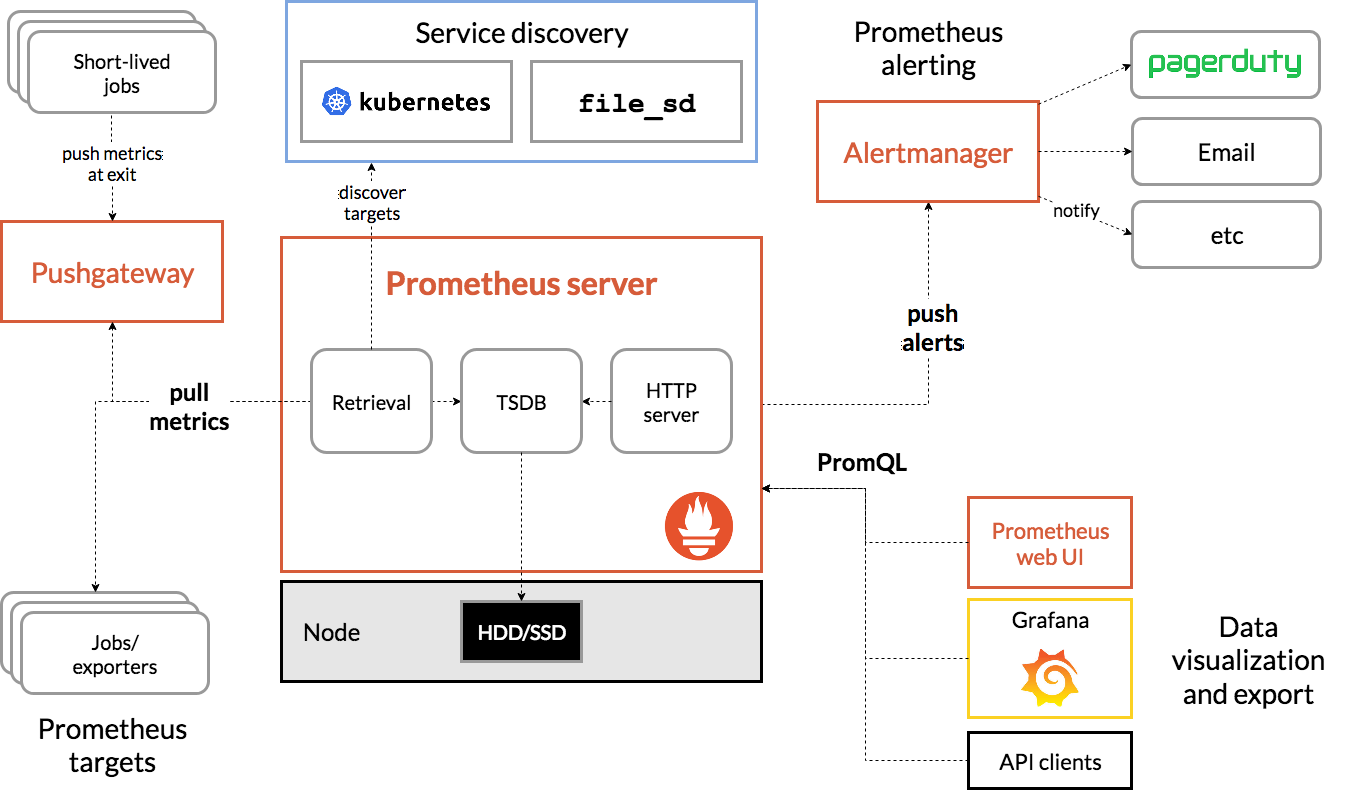
\includegraphics[width=\textwidth]{../assets/prometheus_architecture.png}
  \caption{Prometheus architecture}
  \label{fig:prometheus_architecture}
\end{figure}

\Cref{fig:prometheus_architecture} shows the architecture of Prometheus. Prometheus works by
scraping metrics from instrumented jobs, either directly or through an intermediary push gateway for
ephemeral jobs. It locally stores all scraped metrics and applies rules throughout this data to
enable log aggregation and recording of new time series from existing data or alerts generation.
Afterwards, this time series can be used by Grafana or other API consumers to visualize the
collected data.

Prometheus will be used to scrape and store the metrics of OPNsense VM and Pi-hole container. This
metric will be used by Grafana to create centralised monitoring dashboard.

\subsection{Grafana}

Grafana is an open-source data visualization and monitoring tool used to create interactive and
customizable dashboards for analyzing and monitoring various data sources. It allows users to query,
visualize, and understand data from different systems and applications through a unified and
intuitive interface.

In this project, Grafana will be used to create centralised monitoring dashboard. This includes
VM and container system metrics, network access log, firewall action log, and DNS block log. This
centralised monitoring dashboard allows system administrator monitors the proposed system simpler
and easier.

\section{System Requirement}

This section refers to the process of identifying and specifying the hardware, software, and network
requirements for a particular system or software application. It involves understanding the
necessary resources and capabilities that a system needs to operate effectively and efficiently.

To ensure that the proposed system met the project objectives and able to deliver its functionality
as optimal as possible, several requirements have been determined.

\subsection{Hardware Requirement}

% The main objective of this project is to develop a low-cost hardware firewall by utilizing an old
% PC. As PC is becoming more accessible to every person, it is chosen as the base hardware which the
% firewall and additional application will be deployed.

\begin{table}[H]
  \begin{tblr}{width=\textwidth,colspec={|X[c,m]|X[l,m]|X[l,m]|}}
    \hline
    \SetCell[c=1]{c} Hardware & \SetCell[c=1]{c} Specification & \SetCell[c=1]{c} Justification \\
    \hline
    Laptop & {OS: Windows 11 64-bit \\ CPU: AMD Ryzen 7 4800H 8c16t \\ RAM: 32GB DDR4 \\ Storage:
    2TB NVME SSD} & Environment for project research, development, and maintenance with the
    specified hardware is required to for smooth development \\ 
    \hline
    Proposed System Host & {OS: Proxmox VE 64-bit \\ CPU: Intel Core i5 8600T 6c6t \\ RAM: 16GB DDR4
    \\ Storage: 512GB NVME SSD, 512GB SATA HDD} & Environment for project research, development, and
    maintenance with the specified hardware is required to for smooth development \\ 
    \hline
  \end{tblr}
  \caption{Hardware requirements}
  \label{table:hardware_requirements}
\end{table}

\Cref{table:hardware_requirements} shows the hardware requirements for both laptop to help with
development phase and proposed system host.

\subsection{Software Requirement}

\begin{table}[H]
  \begin{tblr}{width=\textwidth,colspec={|X[c,m]|X[l,m]|}}
    \hline
    \SetCell[c=1]{c} Software & \SetCell[c=1]{c} Justification \\
    \hline
    Neovim & IDE and Documentation writing \\
    Ventoy & Creation of bootable USB \\
    Ansible & Configuration management / Infrastructure as Code \\
    TeX Live & Documentation writing \\
    Google Chrome & Access web GUI of proposed system \\
    Windows Subsystems for Linux & Subsystem to run Linux on Windows \\
    \hline
  \end{tblr}
  \caption{Software requirements}
  \label{table:software_requirements}
\end{table}

\Cref{table:hardware_requirements} shows the hardware requirements for both laptop to help with
development phase and proposed system host.

\section{Summary}

This chapter discussed the detailed steps for the implementation or developments of the proposed
system. Technologies and system requirement which covers both hardware and software requirements are
defined further. Clearly defining the methodology and system requirements will help to ensure the
project is completed and its objectives and deliverable are achieved within the allocated period.
The system requirement, both software and hardware, also discussed for the purpose of keeping the
system running optimally. This chapter discussed the detailed steps for the implementation or
developments of the proposed system. Technologies and system requirement which covers both hardware
and software requirements are defined further. Clearly defining the methodology and system
requirements will help to ensure the project is completed and its objectives and deliverable are
achieved within the allocated period. The system requirement, both software and hardware, also
discussed for the purpose of keeping the system running optimally.

\end{document}
